% !TeX root = ./0_slides.tex

\begin{frame}{STM32 boot: summary}
	\vspace{-3mm}
	\begin{table}[]
		\centering
		\begin{tabular}{|l|l|l|l|l|l|}
			\hline \rule{0pt}{12pt} IC n\textsuperscript{o} & $\bar{\beta_0} \; (^{\circ} C/s)$ & $\sigma_{\beta_0} \; (^{\circ} C/s)$ & $\bar{R^2} \; (^{\circ} C/s)$ & $\sigma_{R^2} \; (^{\circ} C/s)$ & Backside \\ \hline
			25       & 0.931  & 0.229  & 0.011    &  0.005    & Closed           \\ \hline
			3         & 1.405  & 0.145  & 0.06      &  0.015    & Closed            \\ \hline
			12       & 1.819  & 0.204  & 0.18      &	0.085  & Closed            \\ \hline
			6         & 2.183  & 0.191  & 0.08      &	0.012   & Closed            \\ \hline
			2         & 2.503  & 0.322  & 0.174    &  0.146    & Closed            \\ \hline
			26       & 2.97    & 0.16    & 0.057    &  0.006    & Closed            \\ \hline
			1         & 3.433  & 0.159  & 0.093    &  0.08      & Opened         \\ \hline
			9         & 3.965  & 0.167  & 0.336    &  0.021    & Opened         \\ \hline
			10       & 4.341  & 0.193  & 0.144    &  0.1        & Opened         \\ \hline
			7         & 4.567  & 0.137  & 0.278    &  0.023    & Opened         \\ \hline
			8         & 4.843  & 0.222  & 0.232    &  0.086    & Opened         \\ \hline
			4         & 6.351  & 0.149  & 0.437    &  0.078    & Opened         \\ \hline
			11       & 6.539  & 0.237  & 0.385    &  0.096    & Opened         \\ \hline
		\end{tabular}
	\end{table}
\end{frame}

\begin{frame}{STM32 boot: heatsink with 7 backside opened ICs}
%	\vspace{-3mm}
	\begin{columns}
		\begin{column}{0.5\textwidth}
			\centering
			Open-air backside
			\begin{table}[]
				\centering
				\begin{tabular}{|l|l|l|}
					\hline \rule{0pt}{12pt} IC n\textsuperscript{o} & $\bar{\beta_0} \; (^{\circ} C/s)$ & $\sigma_{\beta_0} \; (^{\circ} C/s)$  \\ \hline
					1         & 3.433  & 0.159    \\ \hline
					9         & 3.965  & 0.167    \\ \hline
					10       & 4.341  & 0.193    \\ \hline
					7         & 4.567  & 0.137    \\ \hline
					8         & 4.843  & 0.222    \\ \hline
					4         & 6.351  & 0.149    \\ \hline
					11       & 6.539  & 0.237    \\ \hline
				\end{tabular}
			\end{table}
		\end{column}
		\begin{column}{0.5\textwidth}
			\centering
			Heat-sunk backside
			\begin{table}[]
				\centering
				\begin{tabular}{|l|l|l|}
					\hline \rule{0pt}{12pt} IC n\textsuperscript{o} & $\bar{\beta_0} \; (^{\circ} C/s)$ & $\sigma_{\beta_0} \; (^{\circ} C/s)$  \\ \hline
					1         & 0.831  & 0.222    \\ \hline
					9         & 0.976  & 0.172    \\ \hline
					10       & 0.203  & 0.122    \\ \hline
					7         & 1.728  & 0.161    \\ \hline
					8         & 2.771  & 0.853    \\ \hline
					4         & 4.139  & 0.311    \\ \hline
					11       & 2.996  & 0.213    \\ \hline
				\end{tabular}
			\end{table}
		\end{column}
	\end{columns}
\end{frame}

\begin{frame}{STM32 temperature over 72 hours}
%	\vspace{7mm}
	Beginning: 20:00
	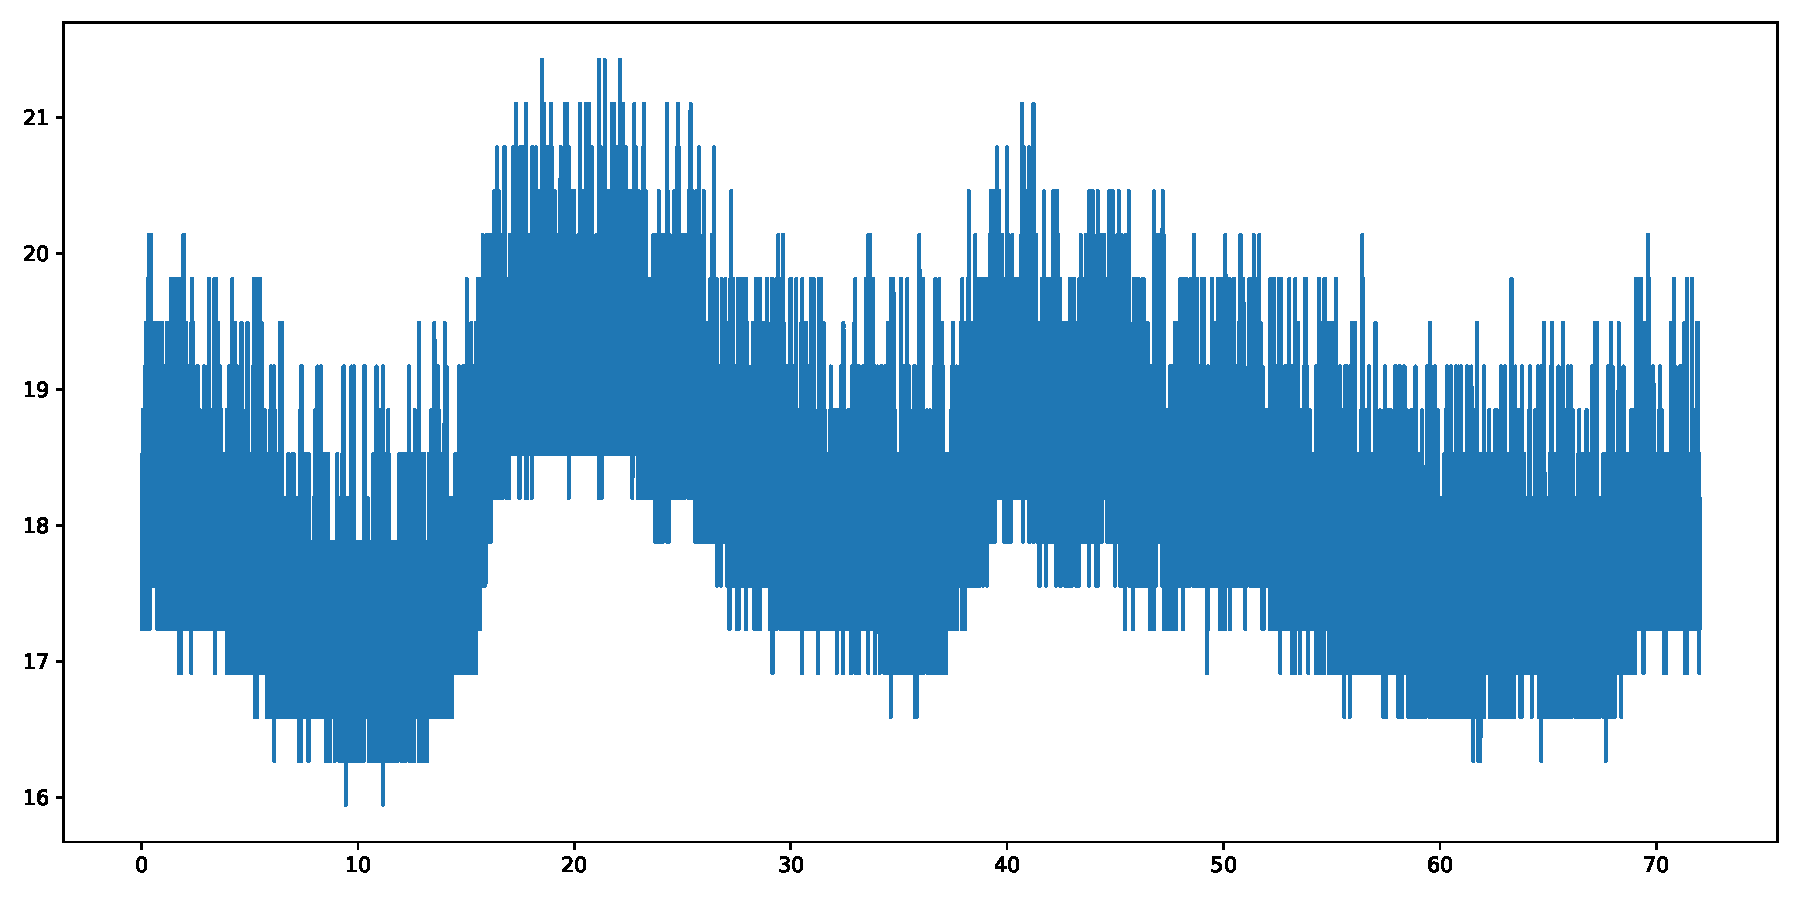
\includegraphics[width=\textwidth]{./figures/temp3days.pdf}
\end{frame}

\begin{frame}{STM32 5 days experiment: Beginning around 16:00 May 7th}
	%	\vspace{7mm}
    \begin{textblock*}{130mm}(2mm, 20mm)
    	\centering
		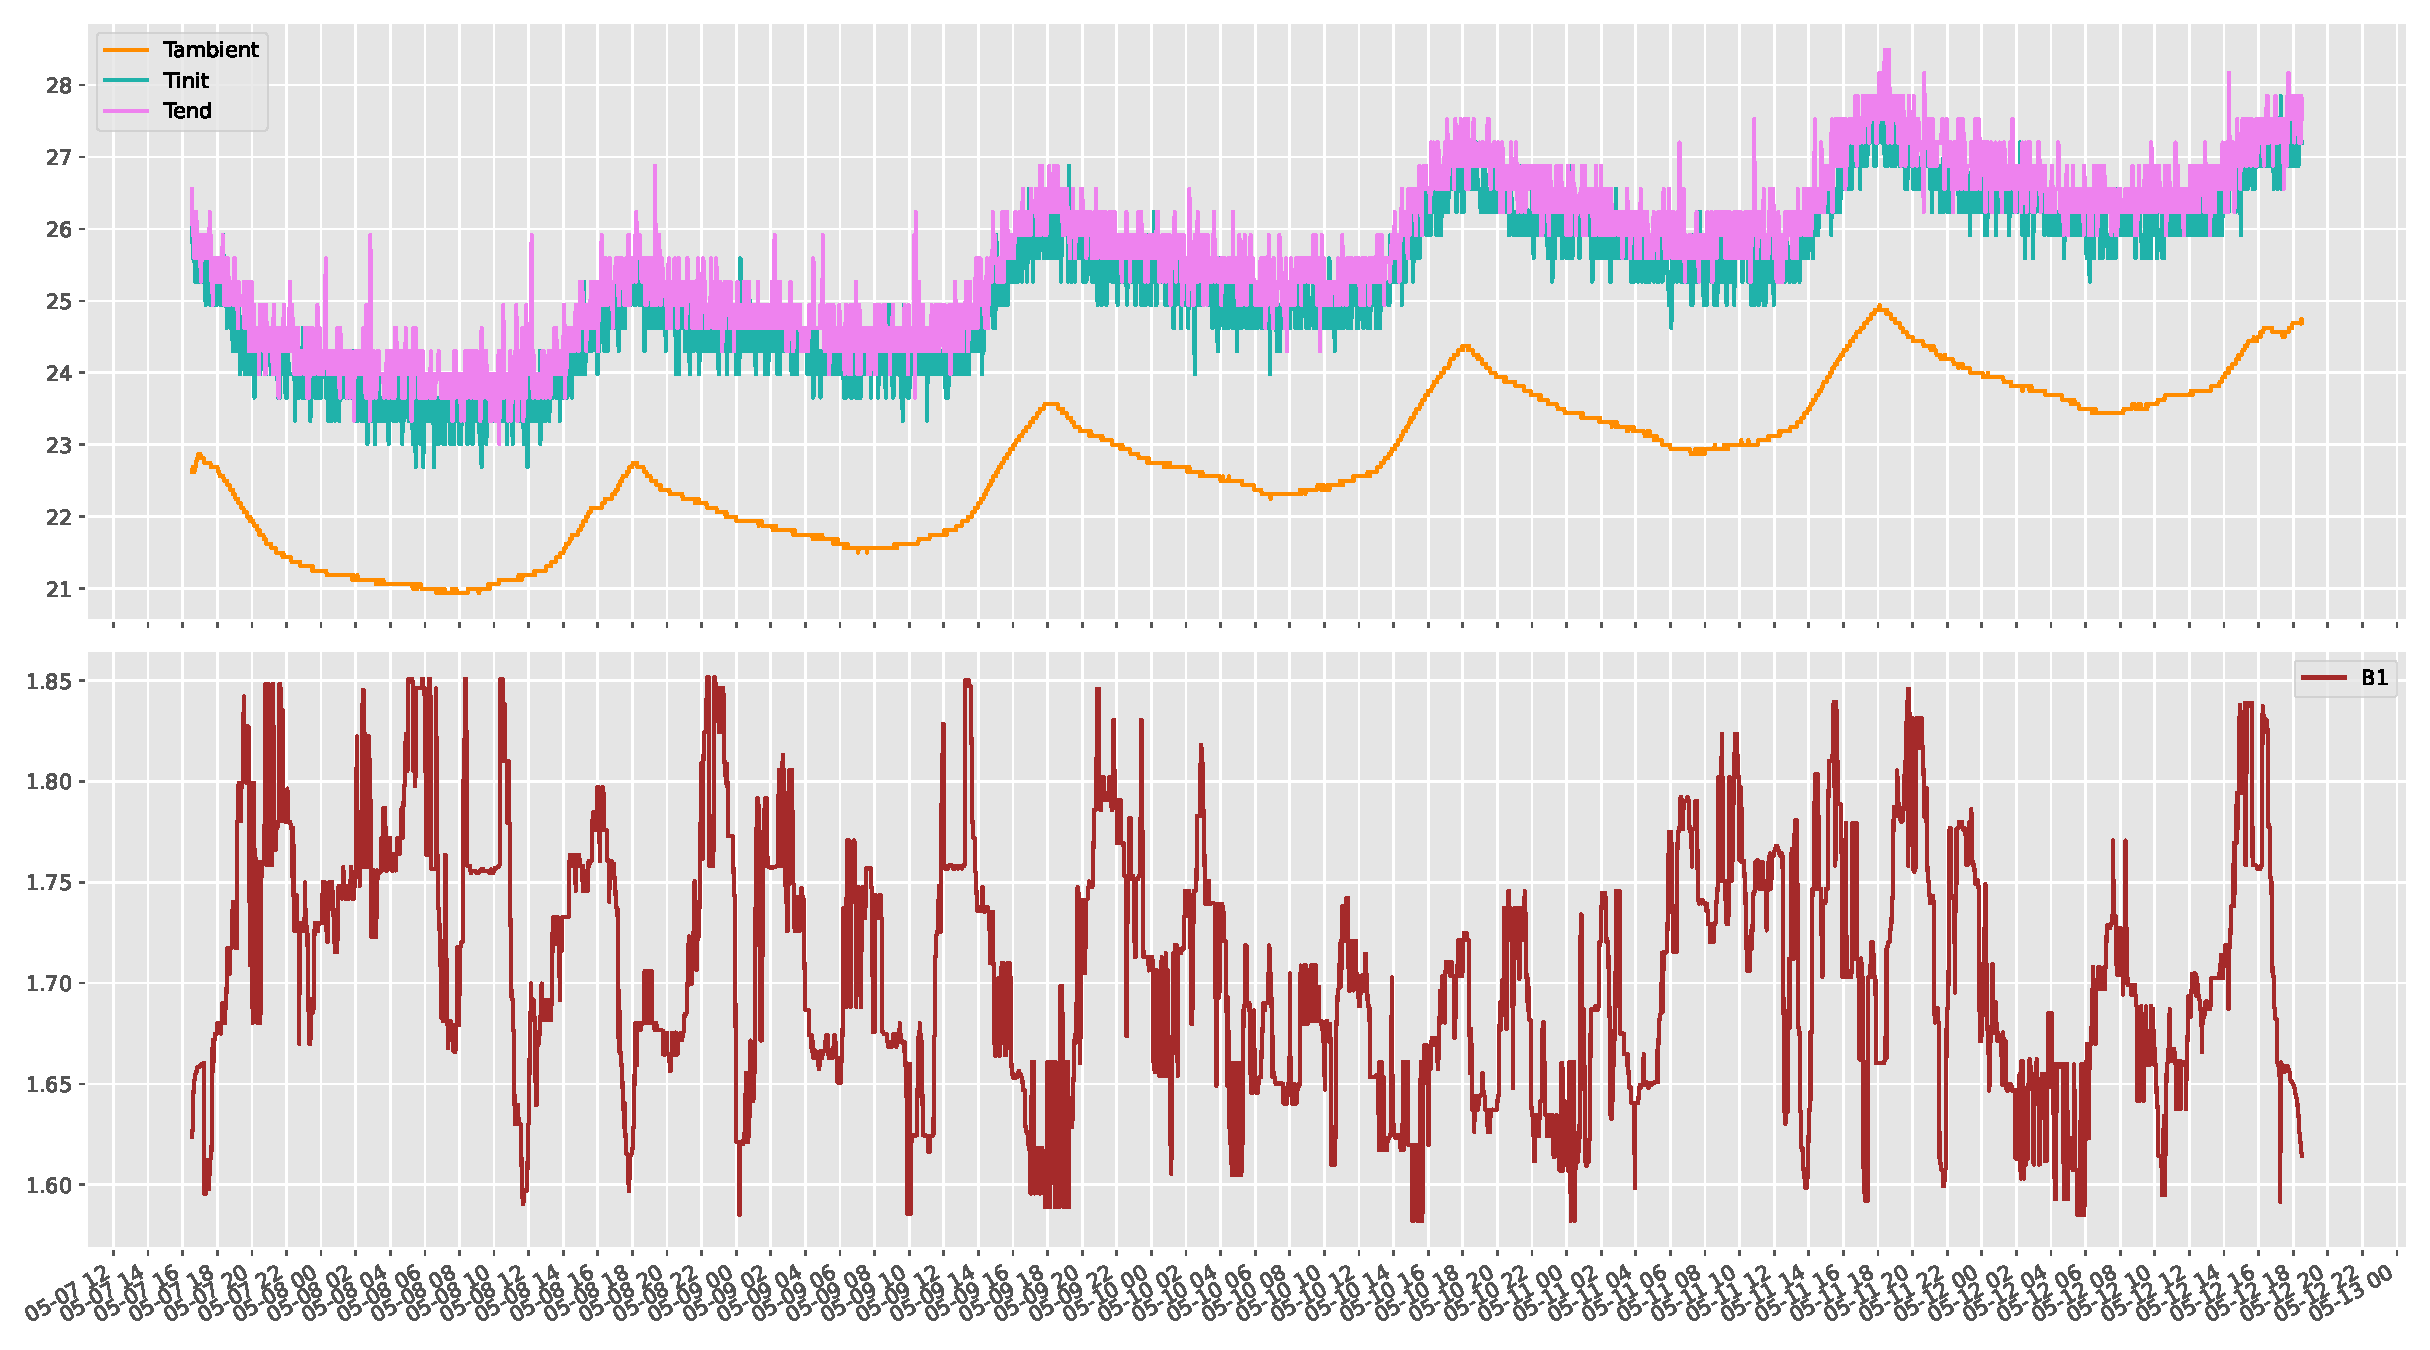
\includegraphics[width=\textwidth]{./figures/stm32_b1_temp_pljours.pdf}
	\end{textblock*}
\end{frame}
